\documentclass[a4paper, titlepage,12pt]{article}
\usepackage[margin=3.7cm]{geometry}
\usepackage[utf8]{inputenc}
\usepackage[T1]{fontenc}
\usepackage[swedish,english]{babel}
\usepackage{csquotes}
\usepackage[hyphens]{url}
\usepackage{amsmath,amssymb,amsthm, amsfonts}
\usepackage[yyyymmdd]{datetime}
\usepackage{listings}
\usepackage{tikz}
\usepackage{xcolor}

\definecolor{codegreen}{rgb}{0,0.6,0}
\definecolor{codepurple}{rgb}{0.5,0,0.5}
\definecolor{backcolor}{rgb}{0.97,0.97,0.97}

\lstdefinestyle{mystyle}{
	commentstyle=\color{codegreen},
	keywordstyle=\color{magenta},
	numberstyle=\color{gray}\ttfamily\footnotesize,
	backgroundcolor=\color{backcolor},
	basicstyle=\ttfamily\footnotesize,
	stringstyle=\color{codepurple},
	numbers=left,
	tabsize=4
}

\lstset{style=mystyle}

\def\ab{.4}
\tikzset{
  net node/.style = {circle, minimum width=2*\ab cm, inner sep=0pt, outer sep=0pt, ball color=blue!50!cyan},
  net node1/.style = {circle, minimum width=2*\ab cm, inner sep=0pt, outer sep=0pt, ball color=red!50!},
  net connect/.style = {line width=1pt, draw=blue!50!cyan!25!black},
  net thick connect/.style = {net connect, line width=2.5pt},
}

\title{Lab NS-3\\Simulation and Performance Analysis of Communication Systems}
\author{Adam Temmel (adte1700)}

\begin{document}
	\maketitle
	\section*{Part 1}\label{sec:introduction}
		\textit{Download from moodle the file} \verb|nineth.cc| \textit{and copy it to your scratch folder. Analyze the code and answer the following questions:}

		\subsubsection*{What is the network topology?}

			The red node represents the recieving node of the system and the blue node represents the source node responsible for sending packets.

			\begin{figure}[h!]
				\centering
				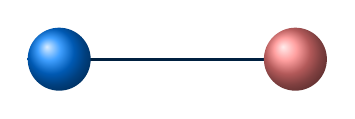
\begin{tikzpicture}
					\path [net connect] (4,0) -- (1,0) node [net node]{};
					\path [net connect] (4,0) -- (4,0) node [net node1]{};
				\end{tikzpicture}
				\caption{The point to point system the lab aspires to simulate}
			\end{figure}

		\subsubsection*{How many queues are used in each node? How are they configured?}

			There are two kinds of queues present in the system, the \verb|DropTailQueue| and the \verb|FifoQueueDisc|. The \verb|DropTailQueue| is used for the packet(s) about to be processed, whereas the \verb|FifoQueueDisc| works as some sort of buffer to contain the packets that do not fit into the prior queue. The \verb|DropTailQueue| is configured to only contain a single packet and the \verb|FifoQueueDisc| is configured to contain 1000 (by default) packets before packets are dropped.

		\subsubsection*{Does the channel introduce errors?}

			No, the channel in itself does not introduce any errors. As far as the channel is concerned, if a packet is inserted into one end, it \emph{will} be extracted in the other end. If the size of the \verb|FifoQueueDisc| is small enough, extracted packets may need to be dropped, meaning that the system can achieve packet loss regardless of the channel being completely intact or not (which, arguably, is a separate question altogether).

		\subsubsection*{How is the traffic generator configured?}

			The traffic generator uses two exponential distributions, one for generating the time between packets (arrival rate) and the size of each packet (departure rate, larger packets take more time to process). The arrival rate distribution has a mean value of $\frac{1}{\lambda}$ and the departure rate distribution has a default mean value of $\frac{1000000}{8\mu}-30$, this is to translate the $\mu$ value given into an appropriate packet size. $1000000$ is the speed of the PTP connection in bits/second, so by dividing it with $8$, we have translated the speed into bytes/second. It is then multiplied by $\frac{1}{\mu}$, akin to the arrival rate distribution. To round it all off, the result is subtracted by $30$, as the header for each packet send is exactly $30$ bytes long.

		\subsubsection*{What are the configuration variables of the code?}

		\begin{figure}[h!]
			\begin{lstlisting}[language=sh]
ns-3-dev % ./waf --run "scratch/nineth --PrintHelp"
Waf: Entering directory `/home/temmel/Documents/ns-3-dev/build'
Waf: Leaving directory `/home/temmel/Documents/ns-3-dev/build'
Build commands will be stored in build/compile_commands.json
'build' finished successfully (2.277s)
nineth [Program Options] [General Arguments]

Program Options:
    --simulationTime:  Simulation time [s] [10]
    --queueSize:       Size of queue [no. of packets] [1000]
    --lambda:          Arrival rate [packets/s] [150]
    --mu:              Service rate [packets/s] [100]
			\end{lstlisting}
		\end{figure}

		\begin{itemize}
				\item \verb|simulationTime| specifies the time the simulation will be running (in terms of "simulator seconds").
				\item \verb|queueSize| specifies the length of the buffer (the FifoQueueDisc).
				\item \verb|lambda| specifies the arrival rate in packets/second.
				\item \verb|mu| specifies the departure rate in packets/second.
		\end{itemize}

		\subsubsection*{What output files are generated?}

			The files that are generated from running the simulation are as follows:

			\begin{itemize}
				\item \verb|ms-lab7-0-0.pcap|
				\item \verb|ms-lab7-1-0.pcap|
				\item \verb|queue.tr|
			\end{itemize}

	\section*{Part 2}
		\subsubsection*{What values should the configuration variables (program arguments) of the code have?}
			\begin{itemize}
				\item \verb|simulationTime| should be set to a number of "okay" size. By increasing the time of the simulation, you also increase the accuracy of the measurements. By setting it to $500$ seconds, the queue.tr file that was generated ended up being almost 5MB, which is more than enough.
				\item \verb|queueSize| should be set to "almost infinite". In this case, a high number is satisfactory enough, meaning that setting it to $100 000$ generated a result with $0\%$ packet loss.
				\item \verb|lambda| should be set to $300$, as specified in the instructions.
				\item \verb|mu| should be set to $330$, as specified in the instructions.
			\end{itemize}

		\subsubsection*{How will you calculate the average buffer size?}
			The \verb|queue.tr| file contains data similiar to:

			\begin{figure}[h!]
				\begin{lstlisting}[language=sh]
1	0
1.001	0
1.002	0
1.003	0
1.004	0
...
1.044	4
1.045	4
1.046	5
1.047	5
1.048	5

				\end{lstlisting}
			\end{figure}

			Where the first column specifies the simulation time, and the second column specifies the number of packets in the queue. As such, calculating the average queue size is equal to calculating the mean value of the second column.

			As such, it is relatively easy to formulate a script that calculates this.\\\\

			\begin{figure}[h!]
				\begin{lstlisting}[language=python]
#!/usr/bin/python

# queue.py

import pandas as pd
import sys

if len(sys.argv) < 2:
    exit(1)

df = pd.read_csv(sys.argv[1], delim_whitespace=True)

warmup = 35
df = df.iloc[warmup:]

print(df["0"].mean())

				\end{lstlisting}
			\end{figure}
			\begin{figure}[h!]
			The script above can be called like:
				\begin{lstlisting}[language=sh]
plots % ./queue.py queue.tr
7.842925577347666
				\end{lstlisting}
			Which gives us a mean value of around $7.8$ packets in the queue.
			\end{figure}
			\subsubsection*{How long should the simulation last?}
				The longer that the simulation runs, the more accurate the calculation of the mean value will be. To some extent, having a too long simulation will effect the calculation time negatively, so an okay balance between the two concepts is ideal. As stated earlier, $500$ seconds ended up producing alright results.

			\subsubsection*{What value of warm-up time will you use?}
				After studying the outputted file, one could notice a lot of leading zeros. By removing these zeros from the mean calculation, we will get a slightly more accurate result. At around 35 logs of the queue size, we encounter our first packet put into the queue, which translates into a warm-up time of $35$ milliseconds.

			\subsubsection*{How many independent simulation runs have you performed?}
				Four separate runs were performed.
				\begin{lstlisting}[language=sh]
plots % ./queue.py queue-1.tr && ./queue.py queue-1-run-1.tr 
	&& ./queue.py queue-1-run-2.tr 
	&& ./queue.py queue-1-run-3.tr
7.842925577347666
7.6181165492901
7.394526276772332
7.9238408728304135
				\end{lstlisting}

		\section*{Part 3}

			\subsubsection*{Compare your findings with results from the mathematical model}

			Running the simulation with a high enough queue size always yields $0\%$ packet loss. We can compare this to the mathematical model:

				\begin{center}
					$P_{100000}=\frac{300}{330}^{100000}\frac{1-\frac{300}{330}}{1-\frac{300}{330}^{100001}} \approx 0$
				\end{center}

			\subsubsection*{Simulate the case with a limited buffer and find the packet loss probability}

				These were the results given after setting the queue size to $8$:

				\begin{figure}[h!]
					\begin{lstlisting}[language=sh]
ns-3-dev % ./waf --run "scratch/nineth 
	--lambda=300 --mu=330 --queueSize=8 --simulationTime=500"
Waf: Entering directory `/home/temmel/Documents/ns-3-dev/build'
[1816/1883] Compiling scratch/nineth.cc
[1849/1883] Linking build/scratch/nineth
Waf: Leaving directory `/home/temmel/Documents/ns-3-dev/build'
Build commands will be stored in build/compile_commands.json
'build' finished successfully (5.899s)

*** Flow monitor statistics ***
  Tx Packets/Bytes:   149879 / 56265782
  Offered Load: 0.902064 Mbps
  Rx Packets/Bytes:   142452 / 53216806
  Packets/Bytes Dropped by Queue Disc:   7518 / 3223778
  Packets/Bytes Dropped by NetDevice:   0 / 0
  Throughput: 0.853187 Mbps
					\end{lstlisting}

					\begin{center}
						$\frac{7518}{149879} \approx 0.0502 = 5.02\%$
					\end{center}

				\end{figure}

			\subsubsection*{Compare your findings with results from the mathematical model}

				\begin{center}
					$P_{8}=\frac{300}{330}^{8}\frac{1-\frac{300}{330}}{1-\frac{300}{330}^{9}} \approx 0.0736 = 7.36\%$
				\end{center}

				We can see that the acquired value and the theoretical value are, indeed, fairly close to each other.
			
			\subsubsection*{Find the value for how long the buffer should be so that the package loss < 1\%}
				
				With some trial and error, having a queue size of $25$, results in a package loss just under 1\%:

				\begin{figure}[h!]
					\begin{lstlisting}[language=sh]
ns-3-dev % ./waf --run "scratch/nineth
	--lambda=300 --mu=330 --queueSize=25 --simulationTime=500"
Waf: Entering directory `/home/temmel/Documents/ns-3-dev/build'
Waf: Leaving directory `/home/temmel/Documents/ns-3-dev/build'
Build commands will be stored in build/compile_commands.json
'build' finished successfully (2.257s)

*** Flow monitor statistics ***
  Tx Packets/Bytes:   149879 / 56265782
  Offered Load: 0.902064 Mbps
  Rx Packets/Bytes:   148917 / 55887156
  Packets/Bytes Dropped by Queue Disc:   975 / 407600
  Packets/Bytes Dropped by NetDevice:   0 / 0
  Throughput: 0.895998 Mbps
					\end{lstlisting}

				\end{figure}
					\begin{center}
						$\frac{975}{149879} \approx 0.0065 = 0.65\%$
					\end{center}

			\subsubsection*{Can you easily calculate this from the mathematical model?}
				
				One could try to use the prior formula, instead solving for $K$. Such an equation would look like:

				\begin{center}
					$P_{k}=0.01=\frac{300}{330}^{k}\frac{1-\frac{300}{330}}{1-\frac{300}{330}^{k+1}} \implies$\\~\\

					$0.01 (1 - \frac{10}{11}^{k+1}) = \frac{10}{11}^k - \frac{10}{11}^{k+1} \implies$\\~\\

					$0.01 - 0.01(\frac{10}{11}^{k+1}+\frac{10}{11}^{k+1}=\frac{10}{11}^k \implies$\\~\\

					$0.01 + 0.99(\frac{10}{11}^{k+1}=\frac{10}{11}^k \implies$\\~\\

					$0.01 = \frac{10}{11}^{k} - 0.99(\frac{10}{11})^k\frac{10}{11} = (\frac{10}{11})^k(1-0.99\frac{10}{11}) \implies$\\~\\

					$\frac{0.01}{(1-0.99\frac{10}{11})} = (\frac{10}{11})^k \implies$\\~\\

					$ln(\frac{0.01}{(1-0.99\frac{10}{11})}) = k \cdot ln(\frac{10}{11}) \implies$\\~\\

					$\frac{ln(\frac{0.01}{(1-0.99\frac{10}{11})})}{ln(\frac{10}{11})} = k = 24.1589$\\~\\

					We cannot have a queue of size 24.1589, so we will have to round it up to 25, giving us the same results as the prior tests.
				\end{center}
				\pagebreak

			\subsubsection*{Modify the simulation to have a M/D/1 queue and compare the results}

				Having a M/D/1 queue means that the departure rate is constant, so the first course of action is to modify the code slightly.

			\begin{figure}[h!]
				\begin{lstlisting}[language=c++]
// New function to generate traffic
static void GenerateTrafficMD1(Ptr<Socket> socket, 
	Ptr<ExponentialRandomVariable> randomTime, double mu) {
    const uint32_t size = (1000000.0/(8*mu)-30);
    socket->Send(Create<Packet> (size));

    Time pktInterval = Seconds(randomTime->GetValue());
    Simulator::Schedule(pktInterval, &GenerateTrafficMD1,
		socket, randomTime, mu);
}

...

// The function is then called once as follows
Simulator::ScheduleWithContext (source->GetNode ()->GetId (),
	Seconds (1.0), &GenerateTrafficMD1, source, randomTime,
	mu);
				\end{lstlisting}
			\end{figure}

			Rerunning the simulator with a "psuedo-infinite" buffer size allows us to find the new average length of the buffer.

			\begin{figure}[h!]
				\begin{lstlisting}[language=sh]
./queue.py queue-2.tr
3.7590449791300706
				\end{lstlisting}
			\end{figure}

			The results suggest that the new average length may lie around 4. This can be investigated further mathematically. 

			\begin{center}
				$E[X^2] = \frac{1}{\mu^2}$\\~\\
				$E[N_q] = \frac{\lambda^2 E[X^2]}{2(1-\rho)} = \frac{300^2 \cdot \frac{1}{330^2}}{2(1-\frac{300}{330}} = \frac{11}{50} \approx 4.595$
			\end{center}

			We can then see that the theoretical values and the simulated results are fairly close to each other.

\end{document}
